\documentclass{article}
\usepackage[utf8]{inputenc}
\usepackage[margin=1in]{geometry}
\usepackage{crop,graphicx,amsmath,array,color,amssymb,flushend,stfloats,amsthm,chngpage,times,fancyhdr,lipsum,lastpage}
\usepackage{subcaption}
\numberwithin{equation}{section}
\usepackage[backend=biber,sorting=none]{biblatex}
\addbibresource{references.bib}

\renewcommand{\bottomfraction}{0.6}

%%%%%%%%%%%%   Header and Footer  %%%%%%%%%%%%%
\pagestyle{fancy}

\fancypagestyle{plain}{%
  \renewcommand{\headrulewidth}{0pt}%
  \fancyhf{}%
  \fancyfoot[R]{Page \bf\thepage\ \rm of \bf\pageref{LastPage}}%
}


%%%% Customise Titles and Headers: %%%%
\title{Project Proposal}
\author{Owen Rowell}
\date{\today}

\fancyhf{}
\fancyhead[L]{Owen Rowell}
\fancyhead[R]{1881130}
\fancyfoot[R]{Page \bf\thepage\ \rm of \bf\pageref{LastPage}}


\begin{document}

%%%%%%%%%%%% Make Title and Format Lines %%%%%%%%%%%%
\maketitle											%
\vspace{-112px}										%
\noindent\rule{\linewidth}{1pt} \par				%
\vspace{100px}										%
\vspace{-20px}										%
\noindent\rule{\linewidth}{1pt} \par				%
\vspace{10px}										%
%%%%%%%%%%%%%%%%%%% Insert Logos %%%%%%%%%%%%%%%%%%%%	
\vspace{-85px}										%
\noindent											%
\begin{minipage}{0.5\textwidth}\begin{flushleft}	%
\hspace{20px}										%

\includegraphics[scale = 0.06]{Resources/UoB}		%
\end{flushleft}\end{minipage}						%
\begin{minipage}{0.5\textwidth}\begin{flushright}	%

\includegraphics[scale = 0.06]{Resources/UoB}		%
\hspace*{20px}										%
\end{flushright}\end{minipage}						%
\vspace{20px}										%
%%%%%%%%%%%%%%%% Headers and Footers %%%%%%%%%%%%%%%%

\begin{abstract}
    
\end{abstract}
\tableofcontents

\newpage
\section{Introduction to Superconductivity}
\subsection{Key phenomena in superconductors}
Superconductivity was discovered by Heike Kamerlinah Onnes in 1911 when he was testing the effect of low temperature on the conduction of electricity in Mercury. He found that when cooled below a critical temperature of $T_c = 4.20K$, the resistance dropped below $10^{-5}\Omega$ - zero to within experimental errors \cite{VanDelft2010TheSuperconductivity}. This phenomenon of perfect conductivity allows a current to flow in a ring without any applied voltage with an experimental lower bound on the half life of $10^5$ years \cite{Tinkham2004IntroductionSuperconductivity}.

Alongside perfect conduction, Meissner and Ochsenfeld also discovered in 1933 superconductors also exhibit perfect diamagnetism in their bulk \cite{Poole2014Superconductivity}. Whilst it could be expected that fields applied to a superconductor are excluded, they also found that any existing fields in the metal as it is cooled below $T_c$ are expelled from the bulk. This phenomena is called the Meissner effect and leads to all superconductors have zero magnetic with only an exponentially decaying "skin" at the boundary. \cite{Tinkham2004IntroductionSuperconductivity}.

As well as superconductors only existing below a material dependent critical temperature $T_c$, the Meissner effect also suggests that in order for the superconductor to be able to retain zero field in the bulk, the external field must also be suitably small. This leads to a critical field $H_c(T)$ above which the superconducting state is destroyed. This critical field is temperature dependent and has the approximate empirical form given by \cite{Tinkham2004IntroductionSuperconductivity}
\begin{equation}
    H_c(T) \approx H_c(0)[1 - (T/T_c)^2].
\end{equation}
It is important to note that the destruction of the superconducting state is unrelated to the source of such a critical field. This means that a field created by the current flowing through the superconductor itself can break superconduction, leading to the idea of a critical current density. For an infinitely long wire this has value \cite{Tinkham2004IntroductionSuperconductivity}
\begin{equation}
    J_c = \frac{H_c}{\lambda}.
\end{equation}
Above this the field at the surface of wire becomes greater than $H_c$ and the medium returns to its normal state.

The two properties of perfect conduction and diamagnetism were described mathematically in 1935 by F. and H. London through two equations now known as the London equations \cite{Poole2014Superconductivity}. These are
\begin{subequations}
\begin{align}
    \nabla \times \mathbf{j} &= -\frac{1}{\mu_0\lambda^2}\mathbf{B} \label{eqn:london1} \\
    \frac{\partial\mathbf{j}}{\partial t} &= \frac{1}{\mu_0\lambda^2}\mathbf{E} \label{eqn:london2},
\end{align}
\end{subequations}
where
\begin{equation}
    \frac{1}{\lambda^2} = \frac{\mu_0n_se^2}{m_e}. \label{eqn:pen_len}
\end{equation}
By substituting in Ampere's law, $\nabla \times \mathbf{B} = \mu_0 \mathbf{j}$, into equation~\ref{eqn:london1}, we get
\begin{align}
    \lambda^2\nabla^2\mathbf{B} &= \mathbf{B}\\
    \implies B &= B_0e^{-\frac{x}{\lambda}}
\end{align}
for a distance $x$ into the superconductor. This mathematically describes the Meissner effect of an exponentially decaying field within the superconductor, characterised by a decay length $\lambda$.

Equation~\ref{eqn:pen_len} relates $\lambda$ to $n_s(T)$, the superconducting electron density. This is the number of electrons per unit volume which exist are able to carry a supercurrent and tends to 0 at $T_c$ leading to a return to the normal state. Similarly, if we consider the boundary of a superconducting and normal metallic state, we could expect to see $n_s$ decay to zero across the boundary according to some characteristic length $\xi(T)$. This can be calculated from Ginzburg-Landau theory, in terms of a temperature dependent parameter $\alpha(T)$ related to the free energy \cite{Tinkham2004IntroductionSuperconductivity}
\begin{equation}
    \xi^2(T) = \frac{\hbar^2}{2m^*|\alpha(T)|}.
\end{equation}
This parameter is called the coherence length and it is this as well as the penetration depth $\lambda$ govern the behaviour of superconductors. Most important is the ratio between these and is called the Ginzburg-Landau parameter \cite{Tinkham2004IntroductionSuperconductivity}
\begin{equation}
    \kappa = \frac{\lambda}{\xi},
\end{equation}
which is responsible for the separation of superconductors in to two distinct types.

\subsection{Type II}
The superconductors discussed so far are more specifically known as type I superconductors and are categorised as those for which $\kappa < \frac{1}{\sqrt{2}}$. In 1957, Abrikosov discovered discovered what are now referred to as type II superconductors \cite{Abrikosov1957TheAlloys}. For values of $\kappa$ of this size, boundaries between normal and superconducting states become preferable to the free energy. This leads to magnetic flux entering the superconductor above a critical field $H_{c1}$ in the form of vortices through the material. These are tubes within which the metal exists in a normal state whilst the superconducting state is retained around it. As the field increases, more of these vortices form to further minimise the free energy through the creation of boundaries, until at some second critical field $H_{c2} = \sqrt{2}\kappa H_c$ the whole material has returned to a normal state.

Ginzburg-Landau theory requires that in order to retain single-valuedness of the order parameter, each vortex must carry an integer number of flux quanta
\begin{equation}
    \Phi_0 = \frac{h}{2e}.
\end{equation}
Since boundaries are energetically preferable, each vortex will carry as little flux as possible, with all other flux forming new vortices. This means that all vortices carry exactly one quantum of flux $\Phi_0$ and larger fields cause more vortices within the medium \cite{Poole2014Superconductivity}. As with any magnetic field, the flux through each vortex induces a supercurrent in the superconducting medium surrounding it. Since such currents then interact with the field in other vortices, a repulsive force is created between the vortices. This repulsion causes the vortices to form a lattice, with this generally being triangular.

It is simplest to study the interaction of these vortices in the high-$\kappa$ limit. This is an acceptable limit in the superconductors such as copper oxides which can have $\kappa \approx 100$. Here the fields from vortices do not overlap and can so can be approximated as a Dirac delta function of flux at the location of the vortex. Adding this term on to the first London equation (equation~\ref{eqn:london1}) and solving gives the field due to one vortex to be \cite{Poole2014Superconductivity}
\begin{equation}
    B(r) = \frac{\Phi_0}{2\pi\lambda^2}K_0\left(\frac{r}{\lambda}\right),
\end{equation}
where $K_0(z)$ is the modified Bessel function of the first kind with order zero. The current induced by this vortex is then found using Maxwell's equation
\begin{align}
    \mathbf{J} &= \frac{1}{\mu_0}\nabla\times\mathbf{B} \nonumber \\
    \implies J(r) &= \frac{\Phi_0}{2\pi\mu_0\lambda^3}K_1\left(\frac{r}{\lambda}\right).
\end{align}
A force is then exerted on other vortices due to the Lorentz interaction between the current and field within the vortex. This gives a vortex on vortex 2 due to vortex 1 as
\begin{equation}
    \mathbf{F}_{21} = f_0K_1\left(\frac{|\mathbf{r}_{12}|}{\lambda}\mathbf{\hat{r}_{12}}\right), \label{eqn:vortex_force}
\end{equation}
where $\mathbf{\hat{r}_{12}}$ is the vector from vortex 1 to vortex 2 and $f_0 = \frac{\Phi_0^2}{2\pi\mu_0\lambda^3}$. It is this interaction and the interaction of vertices with external forces, that will drive the investigations within this project.

\section{The vortex channel system}
\subsection{The Lorentz force}
The interaction between vortices due to the Lorentz force has already discussed in the previous section. However, this force can also be exerted due to an applied current flowing through the superconducting bulk. As we have
\begin{equation}
    \mathbf{F}_I = \mathbf{J} \times \mathbf{\Phi_0}, \label{eqn:lorentz_f}
\end{equation}
acting on any given vortex, this independent on the position or motion of all other vortices so can be treated as a constant force $\mathbf{F}_I$ acting on every vortex. The cross product in equation~\ref{eqn:lorentz_f} requires that this force is perpendicular to the flux so will act in the same plane as all other vortex motion due to the vortex-vortex interaction.

This force leads to a flow of vortices through the superconductor perpendicular to the applied current. Such movement induces an electric field that resists the applied voltage, hence breaking perfect conductivity \cite{Tinkham2004IntroductionSuperconductivity}. However, flux flow can be prevented by pinning the vortices in place so that the Lorentz force cannot move them, thus allowing the resistance to stay at 0. Pinning is caused by defects within the superconductor - either naturally occurring or intentionally introduced through doping. As long as the current is low enough that the Lorentz force is below the pinning force, these vortices will remain stationary and a supercurrent is able to flow in the superconducting state around them \cite{Poole2014Superconductivity}.

\subsection{The channel system}
We have now laid out the basis in which the flux vortices move and interact, from this we can create a channel system in which to investigate their behaviour.
First suggested in 1988 by Pruymboom et al., the channel is made by pinning vortices in the superconductor in their ground state lattice, except for a channel of vortices that are left free to flow. Experimentally, Pruymboom achieved this by placing a layer of NbN, which exhibits strong pinning, on top of a layer of amorphous Nb$_3$Ge, which has weak pinning. Due to the thinness of the layers, the vortices pinned in the the NbN layer continue through the Nb$_3$Ge with little deviation, hence effectively pinning them within the Nb$_3$Ge as well. By cutting channels in the NbN layer, this removes the strong pinning leaving a channel of free flowing flux vortices \cite{Pruymboom1988Flux-lineFilms}.

Figure~\ref{fig:channel_system} shows a section of this system in the simplest case of a channel with width 2 lattice spacings and therefore 1 line of free vortices.
\begin{figure}[htb]
    \centering
    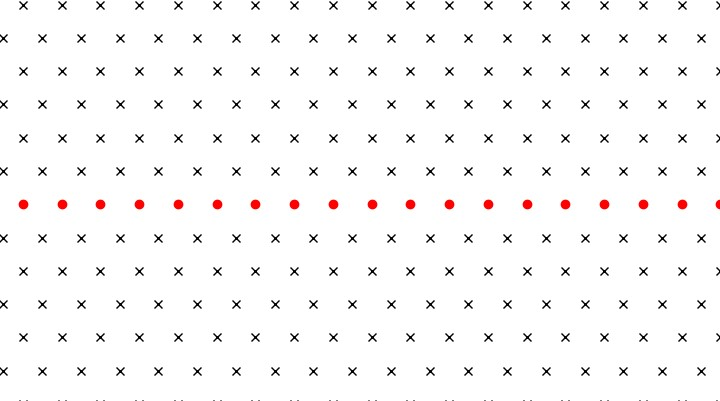
\includegraphics[width=0.8\linewidth]{results/Figures/channel_drawing - cropped.jpg}
    \caption{The channel system with width 1 - crosses represent pinned vortices and red dots represent vortices free to flow along the channel.}
    \label{fig:channel_system}
\end{figure}
In reality, this is a 3d system with the vortices coming out of the page though the block of superconductor. However, as long as the weakly pinning layer is thin, we only need to consider a single 2d plane as the position of the vortices will not vary much through the system \cite{Gartlan2020NovelFibres}.
 
\subsection{Critical shear}
An important quantity of the channel system is the critical shear - the minimum force from the applied current required for the vortices to flow along the channel. For forces below this, the vortices will remain in the wells of the washboard potential created by the pinned vortices as shown in figure~\ref{fig:washboard_f0}. The addition of the constant Lorentz force is a linear increase to the potential causing these wells to "tip", thus reducing there size. Eventually, for some $\mathbf{F}=\mathbf{F}_c$, the potential wells cease to be wells at all and the vortices will begin to flow along the channel as seen in figure~\ref{fig:washboard_fc} \cite{Gartlan2020NovelFibres, Watkins2016DensitySuperconductors}. We can also expect that for $\mathbf{F}\gg\mathbf{F}_c$, the original washboard will be negligible compared to the potential due to $\mathbf{F}$ and the vortices will flow as if only driven by the constant Lorentz force.
\begin{figure}[htb]
\centering
\begin{subfigure}[t]{.33\textwidth}
  \centering
  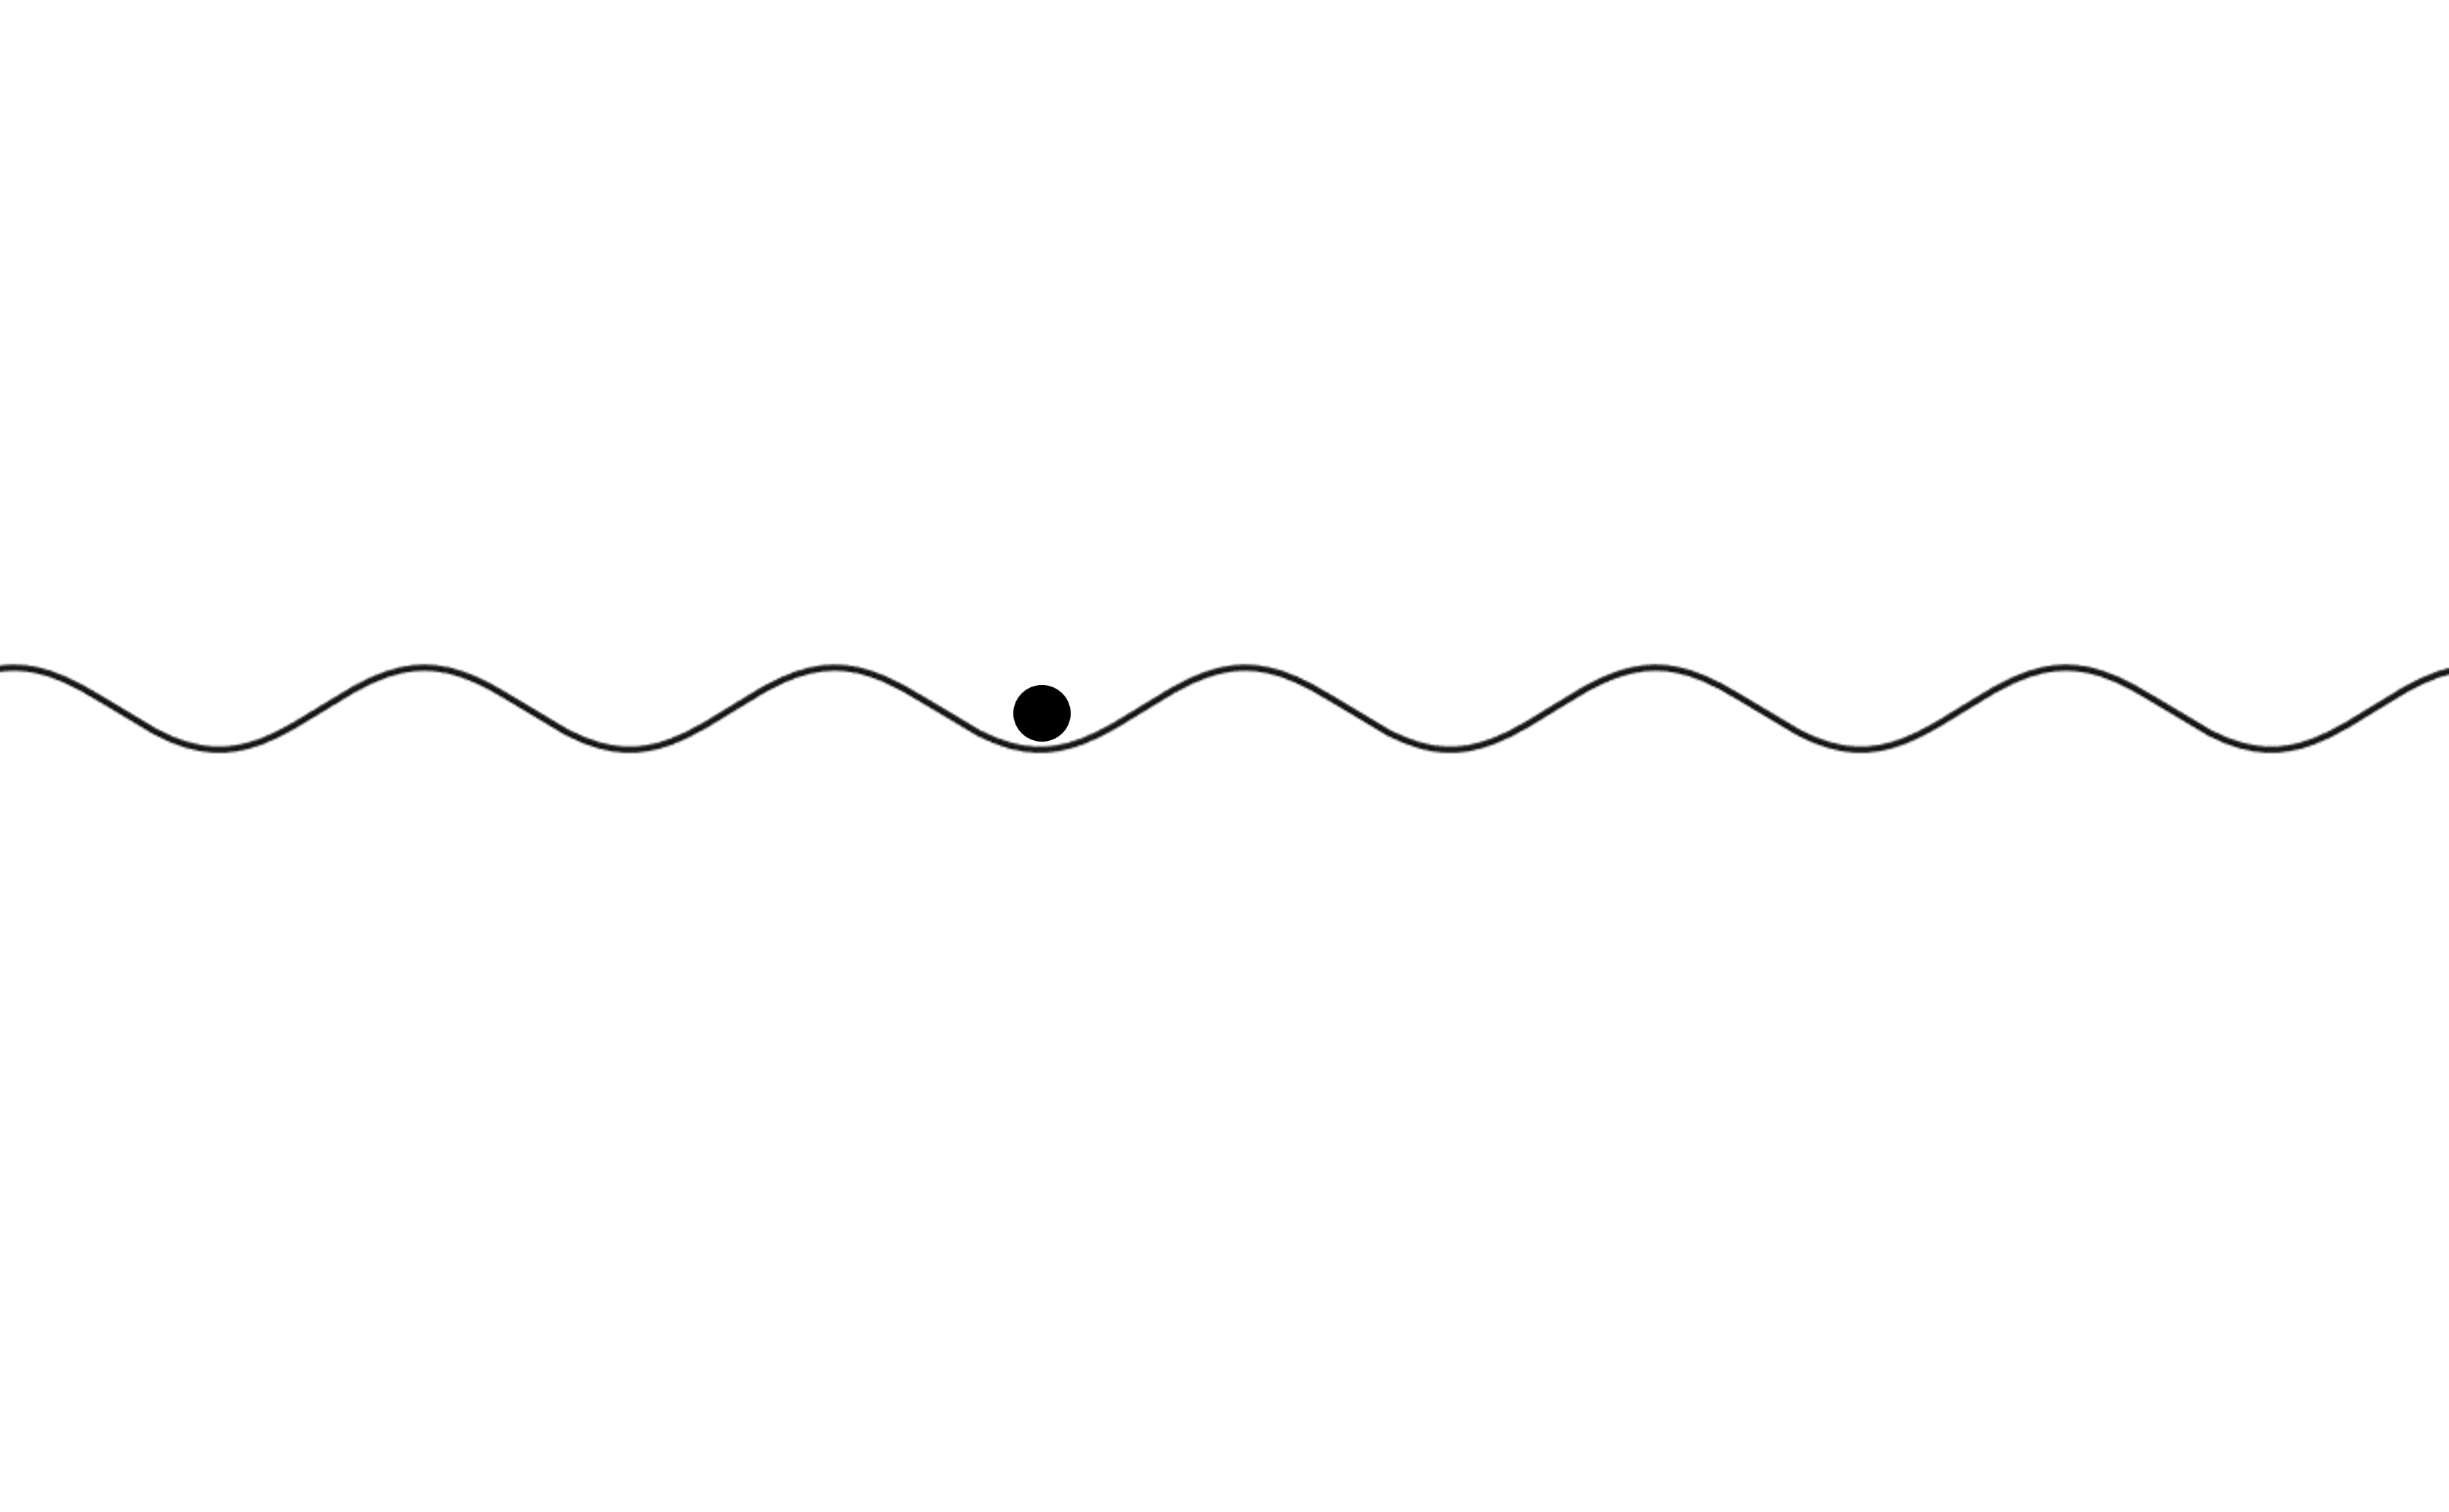
\includegraphics[width=.9\linewidth]{results/Figures/washboard-f0.png}
  \caption{$\mathbf{F}=0$}
  \label{fig:washboard_f0}
\end{subfigure}
\hfill
\begin{subfigure}[t]{.33\textwidth}
  \centering
  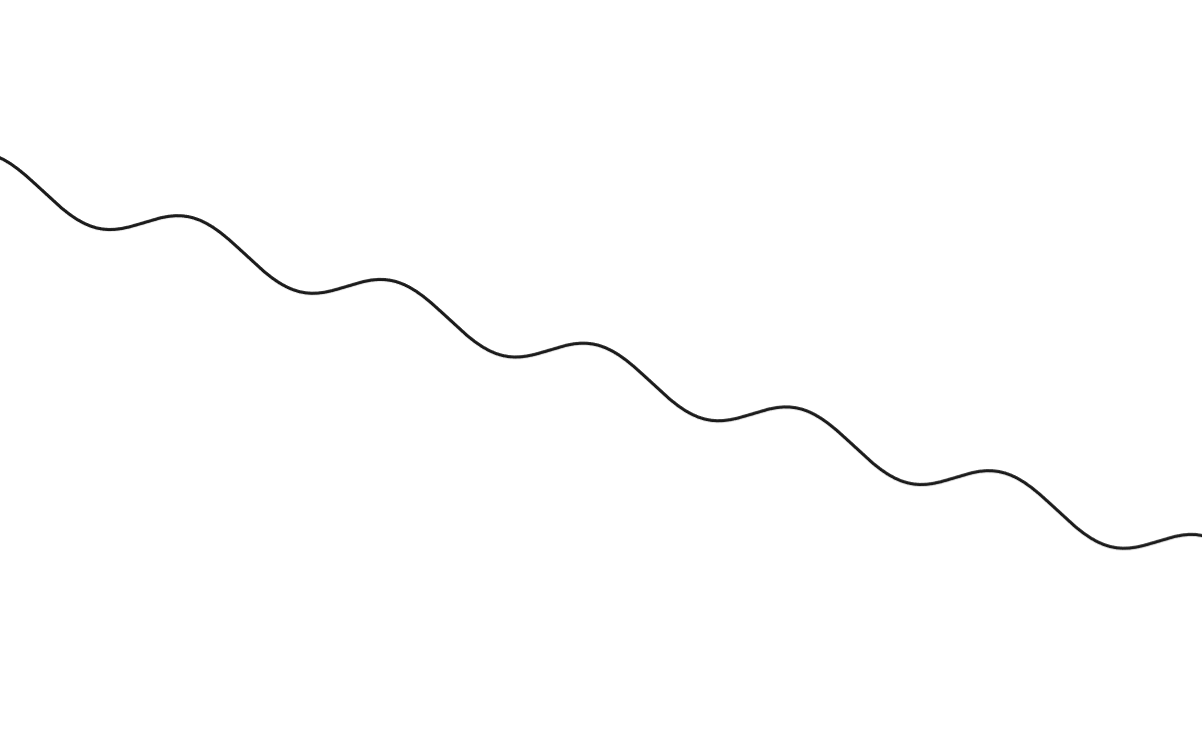
\includegraphics[width=.9\linewidth]{results/Figures/washboard-f.png}
  \caption{$0<\mathbf{F}<\mathbf{F}_c$}
  \label{fig:washboard_f}
\end{subfigure}
\hfill
\begin{subfigure}[t]{.33\textwidth}
  \centering
  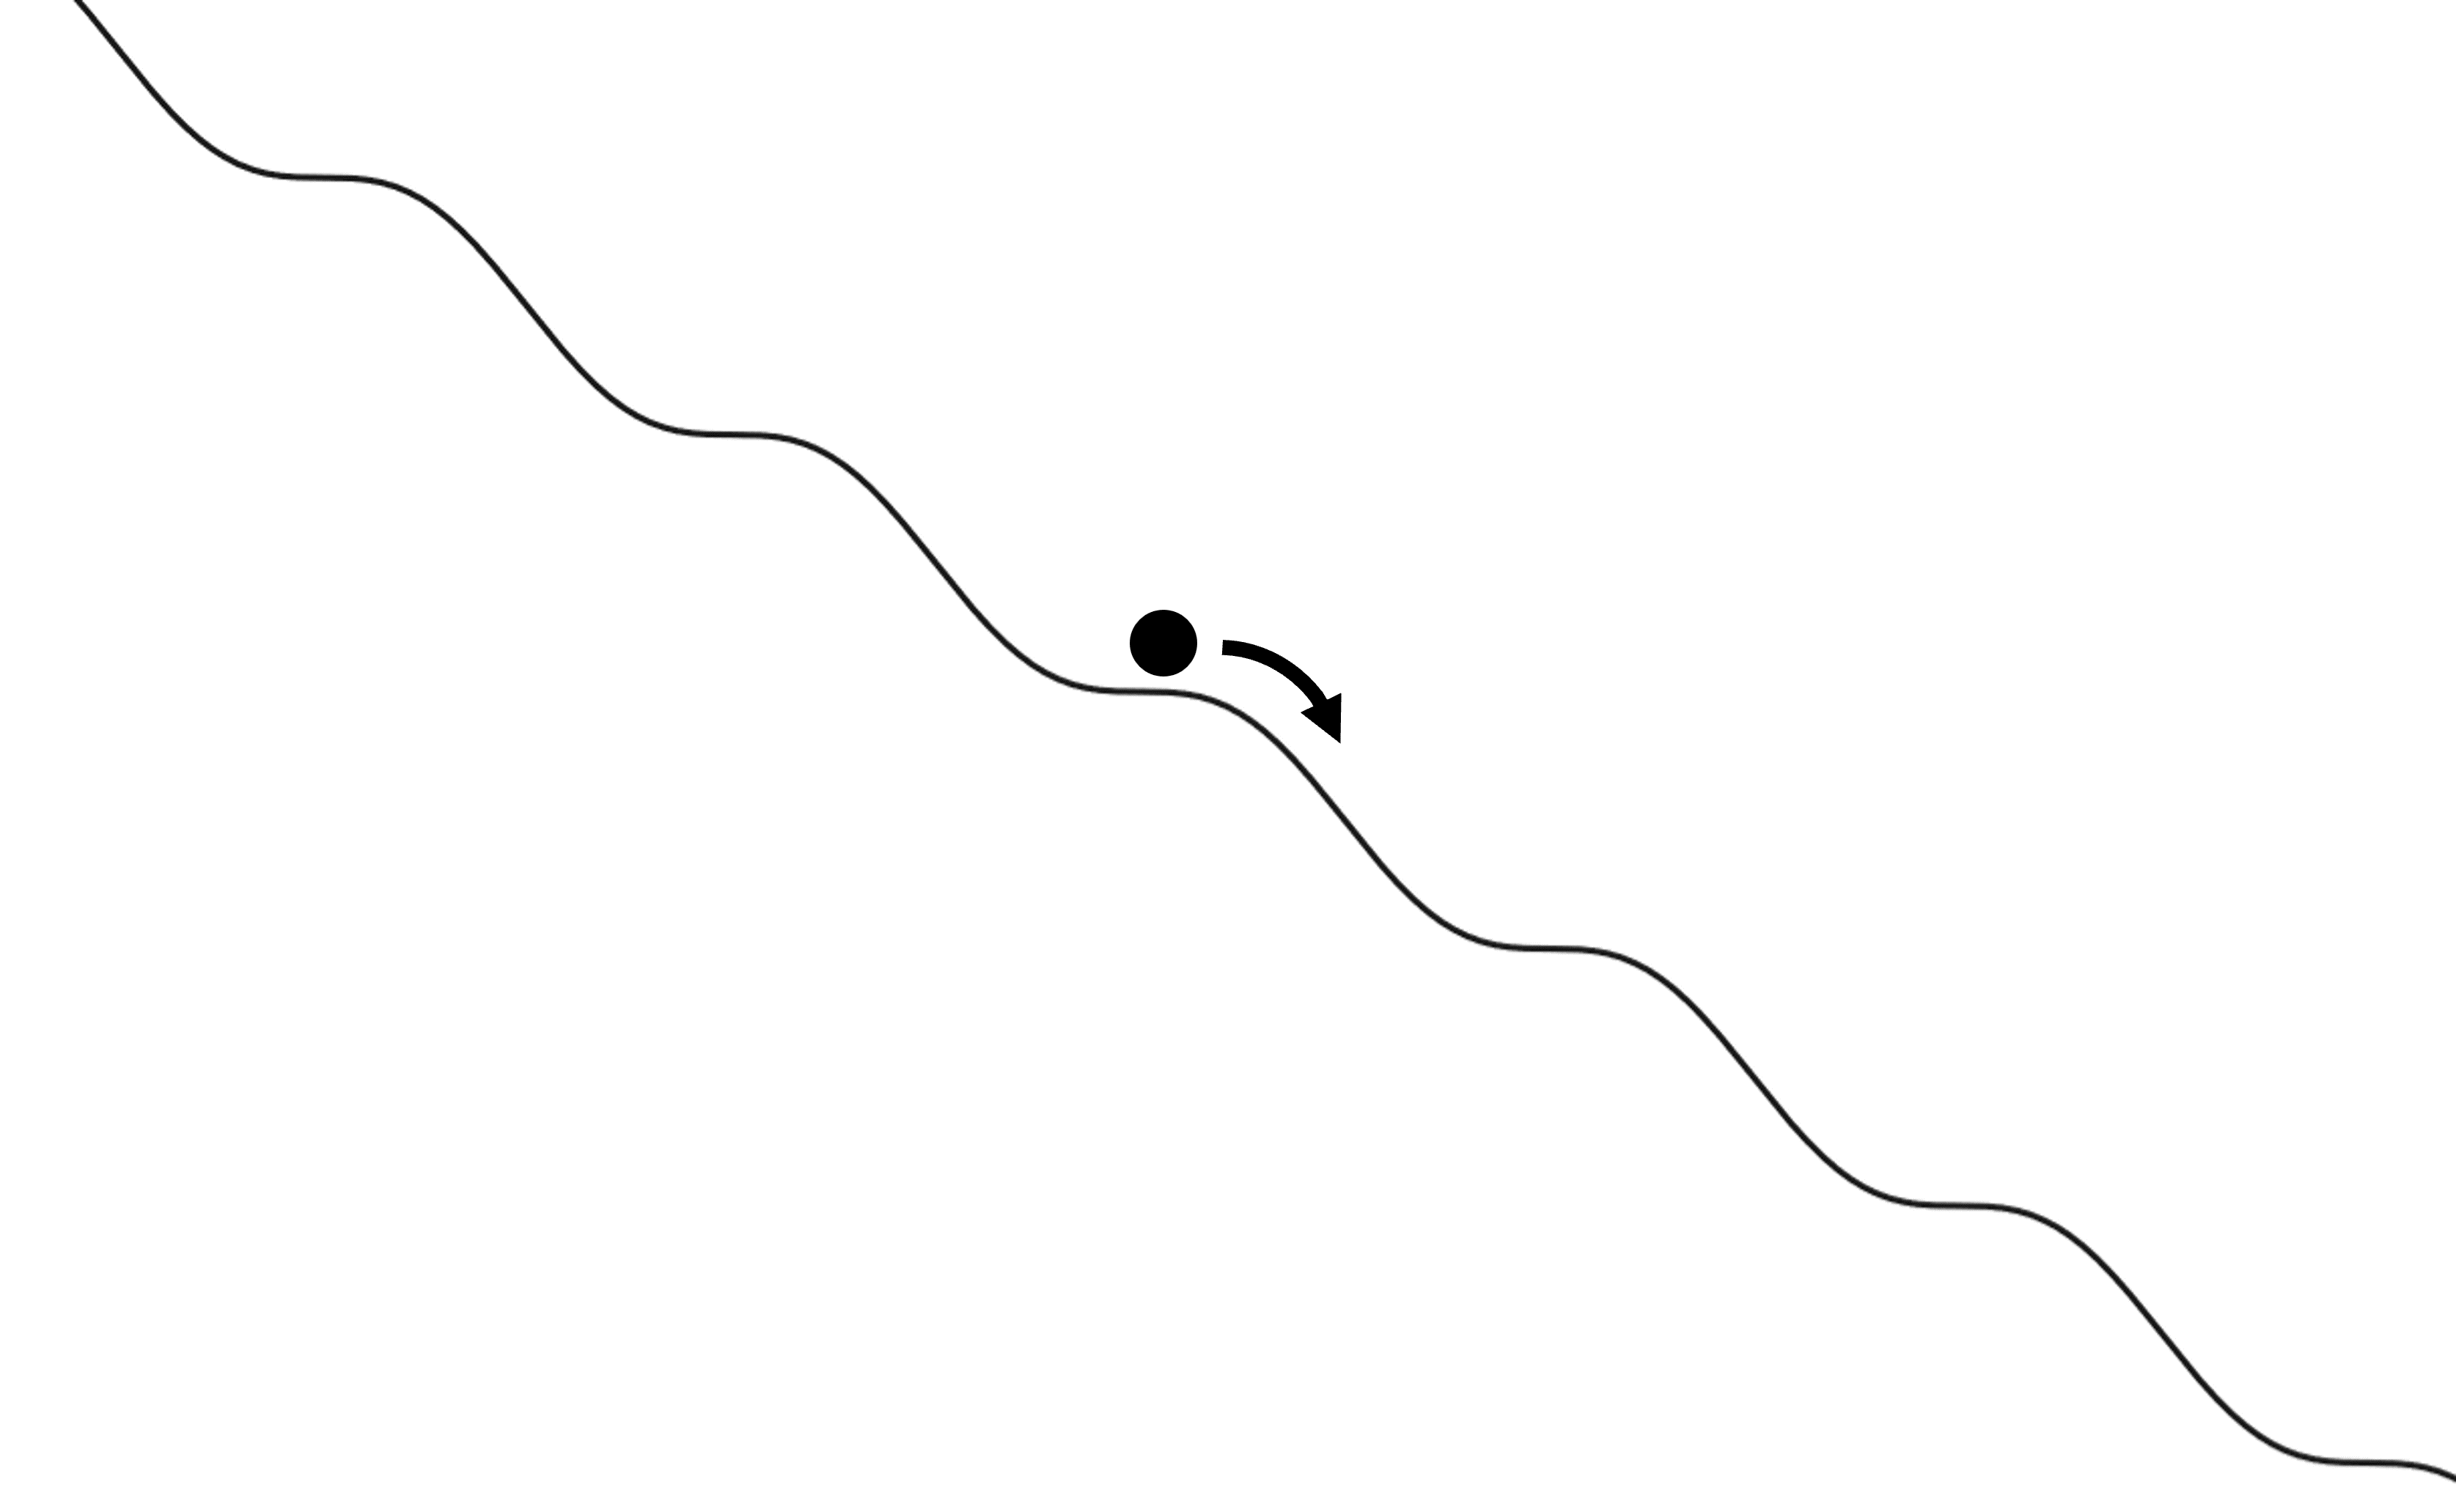
\includegraphics[width=.9\linewidth]{results/Figures/washboard-fc.png}
  \caption{$\mathbf{F}=\mathbf{F}_c$}
  \label{fig:washboard_fc}
\end{subfigure}
\caption{Washboard model of the potential for differing applied forces up to the critical shear}.
\label{fig:washboard}
\end{figure}

This quantity is a useful one to consider due to it's ease of measurability, both experimentally and numerically as will be seen in section~\ref{sec:comp_crit_chear}. A range of currents can be applied to the system and the long-term motion of the vortices (if any) measured to find a cut off point $\mathbf{F}_c$ followed by a tend towards an asymptote $\mathbf{F} \propto \mathbf{v}$ assuming the existence of a terminal velocity.

\section{Simulation method}
Investigation of the channel system is done by simulating it through the use of molecular dynamics. This is done through integrating the equations of motion for each vortex using python with the numpy package. The Bessel function $K_1$ was provided through the scipy special functions library.
\subsection{Molecular dynamics}
In the case of large-$\kappa$, each vortex can be considered as a particle and we can use the Langevin equation, which in the case of 0 temperature is given by
\begin{equation}
    m\ddot{\mathbf{x}} = \mathbf{F} - \eta\dot{\mathbf{x}}, \label{eqn:langevin}
\end{equation}
where $\eta$ is a viscous drag on a vortex due to dissipative forces such as current flowing through the cores of the vortices which are in a non-superconducting state \cite{Bardeen1965TheorySuperconductors, Watkins2016DensitySuperconductors}. This applies to each free vortex in the system leading to a system of $2N$ coupled differential equations in the case where we take the vortices to be straight throughout the superconductor.

We firstly assume that the effect of this $\eta$ is much greater than that of the inertial term $m\ddot{\mathbf{x}}$, such that we can take $m=0$ so that equation~\ref{eqn:langevin}
\begin{equation}
    \dot{\mathbf{x}} = \frac{1}{\eta}\mathbf{F}. \label{eqn:langevin_ovdamp}
\end{equation}
This is commonly called the over damped Langevin equation and effectively assumes the particles instantly reach terminal velocity \cite{Poole2014Superconductivity}.
Integration of this equation is done using the Euler method to give the iterative equation
\begin{equation}
    \mathbf{x}_{n+1} = \mathbf{x}_n + \frac{\Delta t}{\eta}\mathbf{F}_n,
\end{equation}
where $\Delta t$ is some small time step at which forces are calculated and applied to the vortices.

The total force $\mathbf{F}$ in equation~\ref{eqn:langevin_ovdamp}, can be split into three contributing forces
\begin{equation}
    \mathbf{F} = \mathbf{F}_{vv} + \mathbf{F}_L + \mathbf{F}_I
\end{equation}
where:
\begin{itemize}
    \item $\mathbf{F}_{vv}$ is the force due to the vortex-vortex interaction. This is a sum of each individual force between the vortex being considered and every other vortex in the system as given by equation~\ref{eqn:vortex_force}.
    \item $\mathbf{F}_L$ is the force due to the lattice of pinned vortices. Most simplistically, this force is done by the same calculation as for $\mathbf{F}_{vv}$ however due to the large number of vortex interactions this requires, a more efficient, analytical form can be used instead as which is discussed later in section~\ref{sec:analytic_chan}.
    \item $\mathbf{F}_I$ is the Lorentz force due to the applied current. While this can be calculated using equation~\ref{eqn:lorentz_f}, since this does not vary between vortices or over time, the resulting constant force can instead just be applied to each vortex.
\end{itemize}

\subsection{Optimisations}
Whilst physically, the channel system is very long and so contains many vortices, this is infeasible to simulate numerically. Instead periodic boundary conditions are used at either end of the channel where any particles that flow off the end are wrapped to the other side. In order to reduce end effects this would lead to, multiple of images of the system are produced beyond the periodic boundaries. A force is then applied to each real vortex from the images as well as other real vortices.

The calculation of $\mathbf{F}_{vv}$ (and also $\mathbf{F}_L$ when done vortex by vortex) involves $N^2$ individual calculations of the repulsive force. These each involve calculating the value of the Bessel function $K_0$ which is very computationally expensive. To reduce this, a cutoff is used, beyond which it is assumed that any interactions are negligible and so the force taken to be 0. This means that the number of calls to the Bessel function is now $\sim N$ allowing a larger number of vortices to be simulated. However, since the number of vortices that a given vortex interacts with will grow as $r^2$, a cutoff of 9 lattice spacings was used to ensure that the next shell of discounted vortices is negligible, even if individual vortices closer than this exert very small forces.

To improve precision as well as making the results easier to read, constants are chosen such that the simulation generally works on order $1$. To do this we choose $\lambda = \eta = f_0 = a_x = 1$ which also gives $a_y = \frac{\sqrt{3}}{2}$.

\section{Simulation validation}
It is important to ensure that the simulation that has been written is behaving correctly. This can be done through a few tests that have known results and comparing these to those produced by the code.
\subsection{Ground state}
The first and most simple of these is the production of the ground state. Vortices placed in a triangular lattice with spacing $a_x=1$, $a_y=\frac{\sqrt{3}}{2}$ should remain in this state. Similarly, vortices placed in random locations should also arrange themselves into a triangular lattice.

This is done first with only 4 real vortices placed at $(0, 0)$, $(1, 0)$, $(\frac{1}{2}, \frac{\sqrt{3}}{2})$ and $(\frac{3}{2}, \frac{\sqrt{3}}{2})$ using various numbers of images in each direction. Note that if imaging is done 6 times each way, then a total of $13^2-1=168$ image grids are created. Table~\ref{tab:dist_from_images} shows the effect of the number of images on how closely to the ground state the simulation remained at.
\begin{table}[htb]
    \centering
    \begin{tabular}{c|c}
        Images used & Average distance moved from ground state \\
        \hline
        1 & $1.12\times 10^{-2}$ \\
        2 & $1.59\times 10^{-3}$ \\
        4 & $3.04\times 10^{-5}$ \\
        6 & $5.63\times 10^{-7}$ \\
        8 & $1.03\times 10^{-8}$ \\
        10 & $1.90\times 10^{-10}$ \\
    \end{tabular}
    \caption{Average distance away from the ground state travelled by vortices for differing numbers of image vortices in each direction.}
    \label{tab:dist_from_images}
\end{table}
From this we see that the simulation does in fact remain in the ground state, provided enough images are used. Fewer images reduces accuracy as without the full repulsion of a surrounding ground state lattice, the repulsion between the 4 real vortices will cause them to spread out slightly more than the ground state.



\subsection{Comparison to critical shear} \label{sec:comp_crit_chear}
\subsubsection{Analytical form of the channel lattice} \label{sec:analytic_chan}
Using equation~\ref{eqn:vortex_force}, the potential due to a line of pinned vortices along the x-axis of separation $a_x$ can be written as \cite{Watkins2016DensitySuperconductors}
\begin{equation}
    V_L(x, y) = \frac{f_0}{\lambda}\sum_{n=-\infty}^\infty K_0 \left( \frac{\sqrt{(x + na_x)^2 + y^2}}{\lambda} \right).
\end{equation}
Writing the modified Bessel function using the form found in \cite{I.S.Gradshteyn2015TableProducts}
\begin{equation}
    K_0(z) = \frac{1}{2}\int_0^\infty \frac{\mathrm{d}t}{t}e^{-t-\frac{z^2}{4t}}
\end{equation}
allows the Fourier transform of the potential to be written as (neglecting the proportionality constant)
\begin{align*}
    \tilde{V}_L(k_x, k_y) &= \frac{1}{2}\sum_{n=-\infty}^\infty \int_{-\infty}^\infty\frac{\mathrm{d}x}{\sqrt{2\pi}}e^{ik_xx} \int_{-\infty}^\infty\frac{\mathrm{d}y}{\sqrt{2\pi}}e^{ik_y} \int_0^\infty\frac{\mathrm{d}t}{t}e^{-t-\frac{(x+na_x)^2 + y^2}{4\lambda^2t}} \\
    &= \frac{1}{2}\sum_{n=-\infty}^\infty \frac{\mathrm{d}t}{t}e^{-t} \int_{-\infty}^\infty\frac{\mathrm{d}x}{\sqrt{2\pi}}e^{-\frac{(x+na_x)^2}{4\lambda^2t}+ik_xx}
    \int_{-\infty}^\infty\frac{\mathrm{d}y}{\sqrt{2\pi}}e^{-\frac{y^2}{4\lambda^2t}+ik_yy}.
\end{align*}
Taking $x \rightarrow x - na_x$ and using the known result for the Gaussian integral
\begin{equation}
    \int_{-\infty}^\infty\frac{\mathrm{d}z}{\sqrt{2\pi}}e^{-\frac{z^2}{a}+bz} = \sqrt{\frac{a}{2}}e^{\frac{ab^2}{4}}
\end{equation}
gives
\begin{align*}
    \tilde{V}_L(k_x, k_y) &= \frac{1}{2}\sum_{n=-\infty}^\infty e^{-ina_xk_x} \int_0^\infty\frac{\mathrm{d}t}{t}e^{-t} \sqrt{\frac{4\lambda^2t}{2}}e^{\frac{4\lambda^2t(ik_x)^2}{4}} \sqrt{\frac{4\lambda^2t}{2}}e^{\frac{4\lambda^2t(ikyx)^2}{4}} \\
    &= \lambda^2\sum_{n=-\infty}^\infty e^{-ina_xk_x} \int_0^\infty\mathrm{d}te^{-t}e^{-\lambda^2k_x^2t}e^{-\lambda^2k_y^2t} \\
    &= \lambda^2\sum_{n=-\infty}^\infty e^{-ina_xk_x} \left[\frac{-1}{1+\lambda^2k_x^2+\lambda^2k_y^2} e^{-\left(1+\lambda^2k_x^2+\lambda^2k_y^2\right)t}\right]_0^\infty\ \\
    &= \lambda^2\sum_{n=-\infty}^\infty e^{-ina_xk_x} \frac{1}{1+\lambda^2k_x^2+\lambda^2k_y^2} \cdot e^0 \\
    &= \sum_{n=-\infty}^\infty \frac{e^{-ina_xk_x}}{\frac{1}{\lambda^2}+k_x^2+k_y^2}.
\end{align*}
This is then Fourier transformed back using the formula for the Dirac comb
\begin{equation}
    \sum_{n=-\infty}^\infty\delta(k-Tn) = \frac{1}{T}\sum_{n=-\infty}^\infty e^{\frac{2\pi ikn}{T}}.
\end{equation}
This gives
\begin{align*}
    V_L(x, y) &= \int_{-\infty}^\infty\frac{\mathrm{d}k_x}{\sqrt{2\pi}}e^{-ik_xx} \left(\sum_{n=-\infty}^\infty e^{-ina_xk_x}\right) \int_{-\infty}^\infty\frac{\mathrm{d}k_y}{\sqrt{2\pi}} \frac{e^{-ik_yy}}{\frac{1}{\lambda^2}+k_x^2+k_y^2} \\
    &= \int_{-\infty}^\infty\frac{\mathrm{d}k_x}{\sqrt{2\pi}}e^{-ik_xx} \left(\frac{2\pi}{a_x}\right)\sum_{n=-\infty}^\infty
    \delta\left(k_x - \frac{2\pi n}{a_x}\right) \int_{-\infty}^\infty\frac{\mathrm{d}k_y}{\sqrt{2\pi}} \frac{e^{-ik_yy}}{\frac{1}{\lambda^2}+k_x^2+k_y^2} \\
     &= \sum_{n=-\infty}^\infty e^{-\frac{2\pi ixn}{a_x}}\frac{1}{a_x} \int_{-\infty}^\infty\frac{e^{-ik_yy}} {\frac{1}{\lambda^2}+\left(\frac{2\pi n}{a_x}\right)^2+k_y^2}\mathrm{d}k_y.
\end{align*}
Letting $Q_n^2 = \frac{1}{\lambda^2} + \left(\frac{2\pi n}{a_x}\right)^2$ and doing the remaining integral gives
\begin{align}
    V_L(x, y) &= \frac{1}{a_x}\sum_{n=-\infty}^\infty e^{-\frac{2\pi in}{a_x}x} \int_{-\infty}^\infty\frac{e^{-ik_yy}} {Q_n^2+k_y^2}\mathrm{d}k_y \nonumber \\
    &= \frac{1}{a_x}\sum_{n=-\infty}^\infty e^{-\frac{2\pi in}{a_x}x}\cdot \frac{\pi}{Q_n}e^{-|y|Q_n} \nonumber \\
    &= \frac{\pi}{a_x}\sum_{n=-\infty}^\infty \frac{e^{-\frac{2\pi in}{a_x}x-Q_n|y|}}{Q_n}.
\end{align}
A semi-infinite sum over this line of vortices is then done to produce a triangular Abrikosov lattice that can form each side of the channel. This is done by increasing both the $x$ and $y$ offset of $V_L$ with each line.
\begin{align*}
    V_A(x, y) &= \sum_{m=0}^\infty V_L\left(x+\frac{ma_x}{2},y+ma_y\right) \\
    &= \frac{\pi}{a_x}\sum_{n=-\infty}^\infty\frac{1}{Q_n}\sum_{m=0}^\infty
    e^{-i\frac{2\pi n}{a_x}x-Q_n|y|}e^{-mn\pi i-Q_nma_y} \\
    &= \frac{\pi}{a_x}\sum_{n=-\infty}^\infty\frac{1}{Q_n}e^{-i\frac{2\pi n}{a_x}x-Q_n|y|} \sum_{m=0}^\infty\left(e^{-n\pi i-Q_na_y}\right)^m \\
    &= \frac{\pi}{a_x}\sum_{n=-\infty}^\infty\frac{1}{Q_n}e^{-i\frac{2\pi n}{a_x}x-Q_n|y|} \frac{1}{1-e^{-i\pi n-Q_na_y}} \\
    &= \frac{\pi}{a_x}\sum_{n=-\infty}^\infty e^{-i\frac{2\pi n}{a_x}x-Q_n|y|} \frac{1}{Q_n}\frac{1}{1-(-1)^ne^{-Q_na_y}}
\end{align*}
Letting $\alpha_n = \frac{1}{Q_n}\frac{1}{1-(-1)^ne^{-Q_na_y}}$ finally gives
\begin{equation}
    V_A(x, y) = \frac{\pi}{a_x}\sum_{n=-\infty}^\infty\alpha_n e^{-i\frac{2\pi n}{a_x}x-Q_n|y|}.
\end{equation}
There are now two cases to consider - those for a channel with an odd or even number of vortices. This is because if there is an even number of vortices across the channel, the pinned lattices either side of the channel must be offset from each other.
In the odd case
\begin{align}
    V_C(x, y) &= V_A(x, y) + V_A(x, w-y) \nonumber \\
    &= \frac{\pi}{a_x}\sum_{n=-\infty}^\infty\alpha_n e^{-i\frac{2\pi n}{a_x}x} \left(e^{-Q_ny}+e^{-Q_n(w-y)}\right), \label{eqn:V_Codd}
\end{align}
where $w = 2a_y, 4a_y, \ldots$ is the channel width.

Similarly, in the even case
\begin{align}
    V_C(x, y) &= V_A(x, y) + V_A(x+\frac{a_x}{2}, w-y) \nonumber \\
    &= \frac{\pi}{a_x}\sum_{n=-\infty}^\infty\alpha_n e^{-i\frac{2\pi n}{a_x}x} \left(e^{-Q_ny}+e^{-i\frac{2\pi n}{a_x}\frac{a_x}{2}}e^{-Q_n(w-y)}\right) \nonumber \\
    &= \frac{\pi}{a_x}\sum_{n=-\infty}^\infty\alpha_n e^{-i\frac{2\pi n}{a_x}x} \left(e^{-Q_ny}+(-1)^ne^{-Q_n(w-y)}\right. \label{eqn:V_Ceven}
\end{align}
So by combining equations~\ref{eqn:V_Codd} and \ref{eqn:V_Ceven}, $V_C$ can be written as
\begin{equation}
    V_C(x, y) = \frac{\pi}{a_x}\sum_{n=-\infty}^\infty\alpha_n e^{-i\frac{2\pi n}{a_x}x} \left(e^{-Q_ny}+\tau_ne^{-Q_n(w-y)}\right), \label{eqn:V_Ccomb}
\end{equation}
with
\begin{equation}
    \tau_n = \left\{
    \begin{array}{ll}
        1 & \textrm{odd channel} \\
        (-1)^n & \textrm{even channel}
    \end{array}
    \right ..
\end{equation}
The summation in equation~\ref{eqn:V_Ccomb} can be split in two using $Q_n = Q_{-n}$, $\alpha_n = \alpha_{-n}$, $Q_0 = \frac{1}{\lambda}$ and $\tau_0 = 1$ to give
\begin{align}
    V_C(x, y) &= \frac{\pi}{a_x} \left[1\cdot\alpha_0\left(e^{-\frac{y}{\lambda}}+e^{-\frac{w-y}{\lambda}}\right) +\sum_{n=1}^\infty\alpha_n\left(e^{-Q_ny}+\tau_ne^{-Q_n(w-y)}\right) \left(e^{-i\frac{2n\pi}{a_x}x}+e^{-i\frac{2(-n)\pi}{a_x}x}\right) \right] \nonumber \\
    &= V_0(y) + \frac{2\pi}{a_x}\sum_{n=1}^\infty\alpha_n\cos\left(\frac{2\pi nx}{a_x}\right) \left(e^{-Q_ny}+\tau_ne^{-Q_n(w-y)}\right),
\end{align}
where
\begin{equation}
    V_0(y) = \frac{\alpha_0\pi}{a_x}\left(e^{-\frac{y}{\lambda}}+e^{-\frac{w-y}{\lambda}}\right).
\end{equation}

\section{\#\#\#Next steps}
\subsection{Self-organising criticality}
\subsection{\#\#\#New system}

\printbibliography

\end{document}
